\section{测量方法}
\label{sec:method}
我们一共挑选了11个分支比较大的所谓的~Cabibbo~允许的强子衰变道
$\Lmodea$, $\Lmodeb$, $\Lmodec$, $\Lmoded$, $\Lmodee$, $\Lmodeaa$, $\Lmodebb$, $\Lmodedd$, $\Lmodeaaa$, $\Lmodeccc$, $\Lmodeddd$~和~1个重建效率比较高的~Cabibbo~压制的$\Lmodee$~\footnote{除非特别说明,否则本文中所指的衰变道均暗含着电荷共轭道在内的。}。
其中$\Ks,\pizero,\Lambda,\Sigma^0$和$\Sigma^+$这些不是稳定可探测粒子,对于这些中间共振态我们选择如表~\ref{tab:interDecay} 所示的重建方式且引用其在PDG中的分支比结果。

\begin{table}
%\footnotesize
\caption{中间共振态的重建方式及其分支比。}
\centering
\begin{tabular}{c|c}
\hline \hline
衰变方式 &分支比(\%) \\ \hline
$\Ks \to \pip\pim$  &    $69.20\pm 0.05$   \\ 
$\pizero \to \gamma\gamma$       &   $98.823\pm 0.034$    \\
$\Lambda \to p\pim$       &   $63.9\pm 0.5$    \\
$\Sigma^0 \to \Lambda\gamma$       &   $100$    \\
$\Sigma^+ \to p\pizero$       &   $51.57\pm 0.30$    \\
%$\omega    \to \pip\pim\pizero$        &    $89.2\pm 0.7$  \\
\hline
\end{tabular}
\label{tab:interDecay}
\end{table}

我们选择使用双标记的方法来对分支比$\mathcal{B}(\LtoXiXisK)$进行测量。这种方法是由MARK III合作组首次提出来的~\cite{mark3a,mark3b}。
简述一下双标记方法的原理:
如图~\ref{fig:topopkpi}所示$\lambdacp\lambdacm$成对产生。
\begin{figure*}[h]
\centering
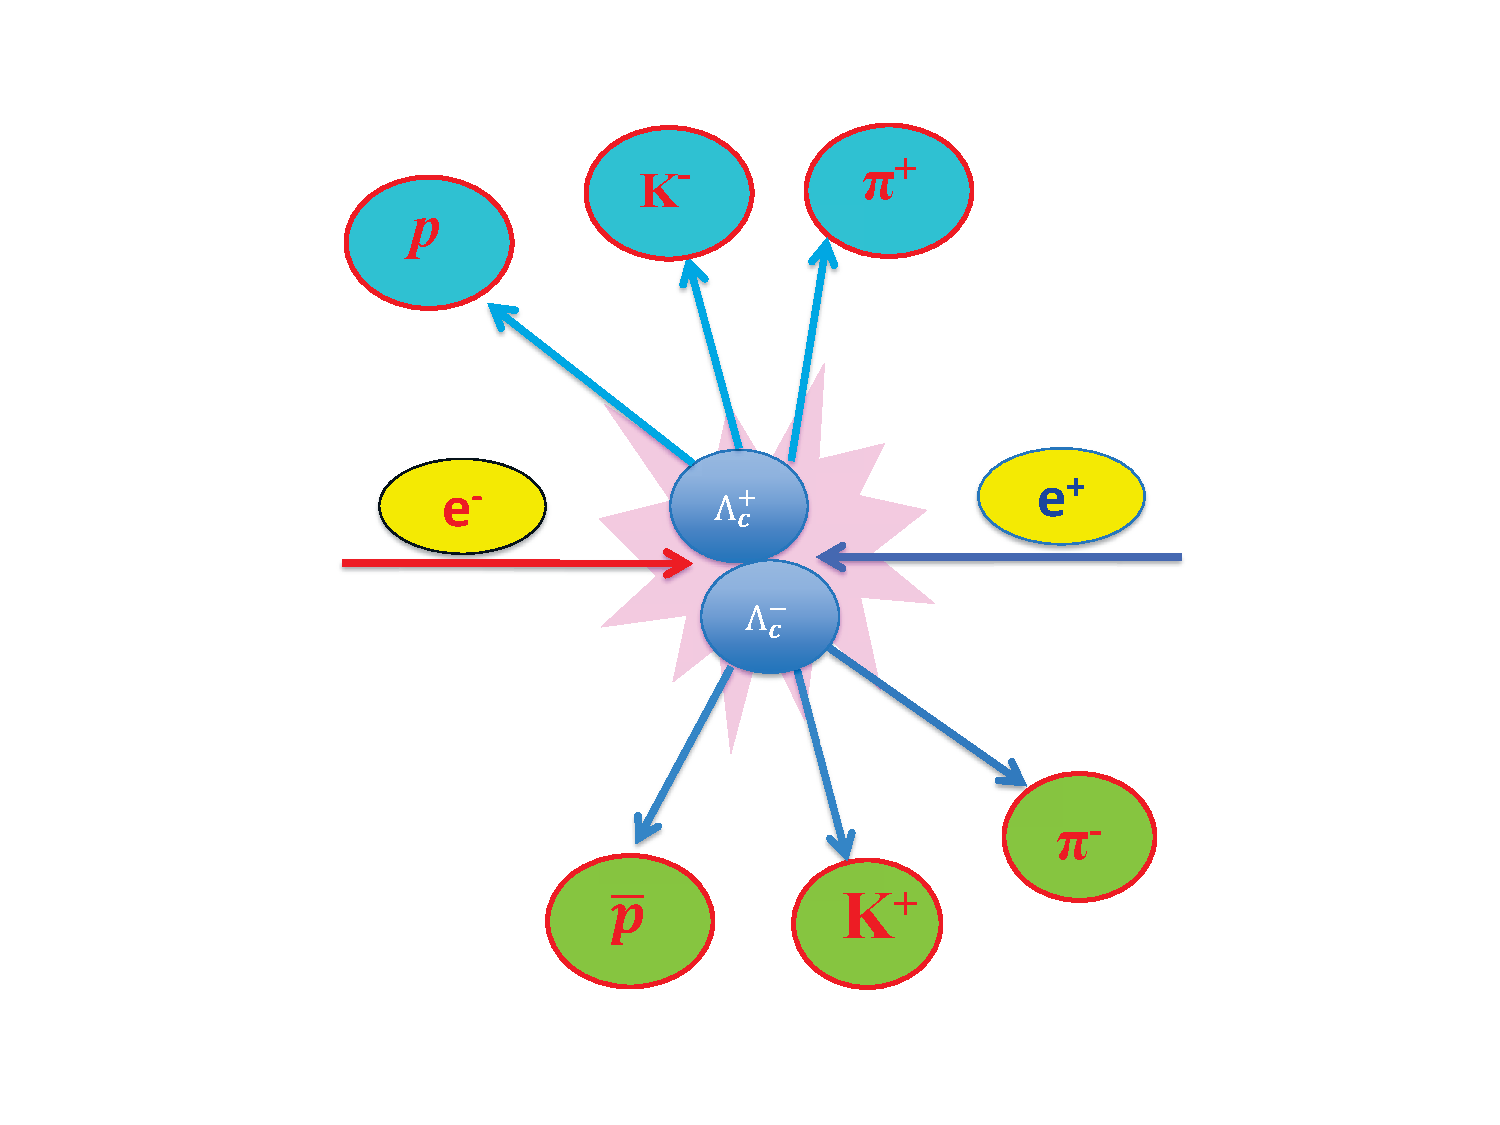
\includegraphics[width=0.4\textwidth]{chap2_topo_pkpi}
\includegraphics[width=0.4\textwidth]{chap2_evtdisplay_pkpi}
\caption{ BESIII 实验上成对产生的$\lambdacp\lambdacm$。 }
\label{fig:topopkpi}
\end{figure*}
我们首先在所有的末态径迹中只重建一个$\lambdacm$,称之为{\it 单标记事例}。
然后我们在单标记$\lambdacm$的反冲侧的末态里面再去重建$\XiXisK$,这称之为{\it 双标记事例}。
则$\LtoXiXisK$的绝对衰变分支比可以通过单标记事例的产额、双标记事例的产额、单标记事例的效率和双标记事例的效率四者之间比例关系求出,
而不需要知道$\lambdacp\lambdacm$事例产生的总数。
举个具体的例子,比如我们想用衰变道$i$作为标记道去测量衰变道$\LtoXiXisK$的分支比。
首先,用$N_{i}^{ST}$来表示$\lambdacp$衰变到这个衰变道$i$的产额,则
\begin{eqnarray}
N_{i}^{\rm ST}&=&N_{\lambdacp\lambdacm}\cdot\mathcal{B}_{i}\cdot\varepsilon_{i}^{\rm ST},
\label{eq:st}
\end{eqnarray}
其中,$N_{\lambdacp\lambdacm}$指的是数据中应有的$\lambdacp\lambdacm$对的总数,
 $\mathcal{B}_{i}$指的是$\lambdacm$衰变到衰变道$i$的分支比,$\varepsilon_{i}^{\rm ST}$指的是这个标记道的重建效率。
对于双标记事例我们指定$\lambdacm \to i$ 并且 $\LtoXiXisK$,故双标记产额$N_{i,\XiXisK}^{\rm DT}$可以表示为:
\begin{eqnarray}
N_{i,\XiXisK}^{\rm DT}&=&N_{\lambdacp\lambdacm}\cdot\mathcal{B}_{i}\cdot\mathcal{B}(\LtoXiXisK)\cdot\varepsilon_{i,\XiXisK}^{\rm DT},
\label{eq:dt}
\end{eqnarray}
其中$\varepsilon_{i,,\XiXisK}^{\rm DT}$指的是$\lambdacm \to i$ 并且 $\LtoXiXisK$同时被重建出的效率,称作双标记效率。
对公式~\ref{eq:st}和公式~\ref{eq:dt}进行简单的代数运算可以得到计算$\LtoXiXisK$的分支比公式:
\begin{eqnarray}
\mathcal{B}(\LtoXiXisK) &=& \frac{N_{i,\XiXisK}^{\rm DT}}{N_{i}^{\rm ST}}\cdot\frac{\varepsilon_{i}^{\rm ST}}{\varepsilon_{i,\XiXisK}^{\rm DT}}.
\label{eq:ratio}
\end{eqnarray}

这种测量分支比的方法称为“ 绝对(absolute)分支比 ” 测量,这种方法的突出优点是:
\begin{itemize}
  \item 不需要知道$\lambdacp\lambdacm$的总数;
  \item $\frac{\varepsilon_{i,\XiXisK}^{\rm DT}}{\varepsilon_{i}^{\rm ST}}$,消掉了很多单标记侧的系统误差,提高了测量的精度。
\end{itemize}

具体到我们这个分析中$\LtoXiXisK$绝对衰变分支比的测量,由于单个双标记产额$N_{i,\XiXisK}^{\rm DT}$的数目太少,所以我们将12个单标记道对应的双标记产额加在一起来处理,将公式\ref{eq:st}和公式\ref{eq:dt}联立并且求和,有如下公式:
\begin{eqnarray}
N_{-,\XiXisK}^{\rm DT}&=&\sum_{i}N_{i,\XiXisK}^{\rm DT}=\mathcal{B}(\LtoXiXisK)\cdot\sum_{i}(\frac{N_{i}^{\rm ST}}{\varepsilon_{i}^{\rm ST}}\cdot\varepsilon_{i,\XiXisK}^{\rm DT}).
\label{eq:br}
\end{eqnarray}
公式\ref{eq:br} 就是我们直接计算分支比的公式。

从上面的讨论中可以看出整个分析流程我们只要知道单标记事例的产额$N_{i}^{\rm ST}$、双标记事例的产额$N_{i,\XiXisK}^{\rm DT}$、单标记事例的效率$\varepsilon_{i}^{\rm ST}$和双标记事例的效率$\varepsilon_{i,\XiXisK}^{\rm DT}$即可对分支比进行计算,接下来的章节就是去阐述怎么去获取上述这些数值。

\section{实验数据和MC模拟样本}
\label{sec:sample}
本分析使用BESIII在BOSS6.6.4p01下重建下的2014年3月份在质心系能量$\sqrt{s}=4.6\gev$处采集的数据,总的积分亮度为567\,pb$^{-1}$~\cite{Ablikim:2015nan}。 

我们使用Monte Carlo (MC)模拟样本来理解本底和估计探测效率。
对于探测器的模拟我们使用非常成熟的GEANT4~\cite{ref:geant4a,ref:geant4b}软件包。
MC模拟的时候我们使用KKMC~\cite{Jadach:2000ir}考虑束流的能散和初态辐射以及带电粒子的末态辐射效应。
为了满足本分析的需要我们模拟产生了如下3类的MC样本:

\begin{itemize}
    \item Cocktail MC 事例: 用来研究本底情况和估计效率。包含BESIII官方产生的MC样本~\cite{pingrg_mc}还有根据我们自己的需求又大量模拟的一些。这里将此类样本总结到表~\ref{tab:MCsample}中,并且列出与数据中该过程的事例数(亮度)比例关系。对于部分QED过程如$\ee$、$\mu^+\mu^-$和$\gamma\gamma$,由于其对我们要研究的衰变过程均无贡献故未列出。需要指出的一点是$\lambdacp\lambdacm$过程是我们最关心的过程,从而进行了大量的模拟且分成了均等的两份:一份用来估计单标记道的重建效率;另一份用来做输入输出检查。
    \item 单标记信号形状MC:顾名思义就是用这份MC样本来获取用来拟合的信号形状。我们要求单标记侧$\lambdacp$ ($\lambdacm$)衰变到12个信号道,另外一侧的$\lambdacm$ ($\lambdacp$)严格地衰变到$e^{-}+\overline{\nu}_{e}$($e^{+}+\nu_{e}$),这样模拟MC的目的是为了得到一份干净的信号MC形状,因为这样另外一侧的末态粒子可以认为是不会对单标记侧造成任何影响的。我们一共模拟了150万个该过程的事例。

    \item 双标记信号MC:用来获取双标记事例的效率。 我们要求两侧的$\Lambda_c$都衰变到12个信号道。由于双标记选择效率较低,为了减小由于模拟统计量有限导致的效率误差我们共产生了大量该过程事例。
\end{itemize}

以上所述各种MC所有涉及$\ee \to \lambdacp\lambdacm$过程的,初态辐射波恩截面是按照BESIII所测结果图~\ref{fig:lambc_cs_bes3}放进EVTGEN考虑了的,并且$\lambdacp$或者$\lambdacm$次级衰变的模型是按照我们在数据中观测到的模式进行模拟的。
\begin{table}
\footnotesize
\caption{Cocktail MC 包含的各个物理过程,相应的截面及其与数据的比例关系。}
\centering
\begin{tabular}{l|c|c|c|c}
\hline \hline
物理  & 截面  & $567\,\rm{pb}^{-1}$的数据 & MC模拟 & MC是数据 \\ 
过程  & (nb)  & 中的事例数($10^6$) & 事例数($10^6$)  & 的倍数 \\ \hline
$\lambdacp\lambdacm$ & 0.178\protect\footnotemark  & 0.1009  & 3.874+3.874  &  38.4+38.4  \\ \hline 
DD & 3.3  & 1.8711  & 4.94  &  2.64  \\ \hline 
qqbar & 16  & 9.072  & 10.9  &  1.2  \\ \hline 
$\tau^+\tau^-$ & 3.4  & 1.9278  & 9  &  4.67  \\ \hline 
ISR 到较轻$\psi$态 & 0.67  & 0.38  & 4  &  10.5  \\ \hline 
\hline
\end{tabular}
\label{tab:MCsample}
\end{table}
\footnotetext{此处截面值为4.6$\gev$处的观测截面,区别于图~\ref{fig:lambc_cs_bes3}中所示波恩截面。}


